\documentclass[11pt]{article}
\usepackage[left=3cm,right=3cm,top=3cm,bottom=3cm]{geometry}
\usepackage{url}
\usepackage{amssymb}
\usepackage{mathrsfs, bm}
\usepackage{amsmath}
\usepackage{enumitem}
\usepackage{array}
\usepackage{graphicx}
\usepackage{booktabs}
\graphicspath{ {./images/} }

\usepackage{titlesec}
\newcommand{\sectionbreak}{\clearpage}

\begin{document}
\title{COMP0123 Complex Networks and Webs Coursework 1 Report}
\author{Roman Ryan Karim}
\date{October 26, 2023}
\maketitle

\section*{Task 1 - (15 marks)}

\fbox{
  \parbox{1\textwidth}{
  \begin{itemize}
	\item Calculate the average node degree and the maximum node degree of the 3 networks.
	\item Plot their degree distribution $P(k)$ on linear-linear scale and log-log scale, respectively.
	\item Estimate the power-law exponent of the degree distribution $P(k)$ of the author network only.
	\begin{itemize}
		\item You can fit a curve by using the function polyfit from the numpy library.
		\item Ideally, you can do the fitting on CCDF (the complementary cumulative distribution function) on log-log scale.
	\end{itemize}
	\item Briefly discuss your results, e.g. difference of the networks.
\end{itemize}}
}

\begin{table}[h]
\centering
\begin{tabular}{lccc}
\toprule
& \textbf{Author Network} & \textbf{Random Network} & \textbf{BA Network} \\
\midrule
Average Degree $\bar{k}$ & 4.99 & 4.99 & 4.99 \\
Maximum Degree $k_{max}$ & 51 & 14 & 82 \\
Power-Law Exponent $\alpha$ & 2.01 & & \\
\bottomrule
\end{tabular}
\end{table}

\begin{figure}[h]
    \centering
    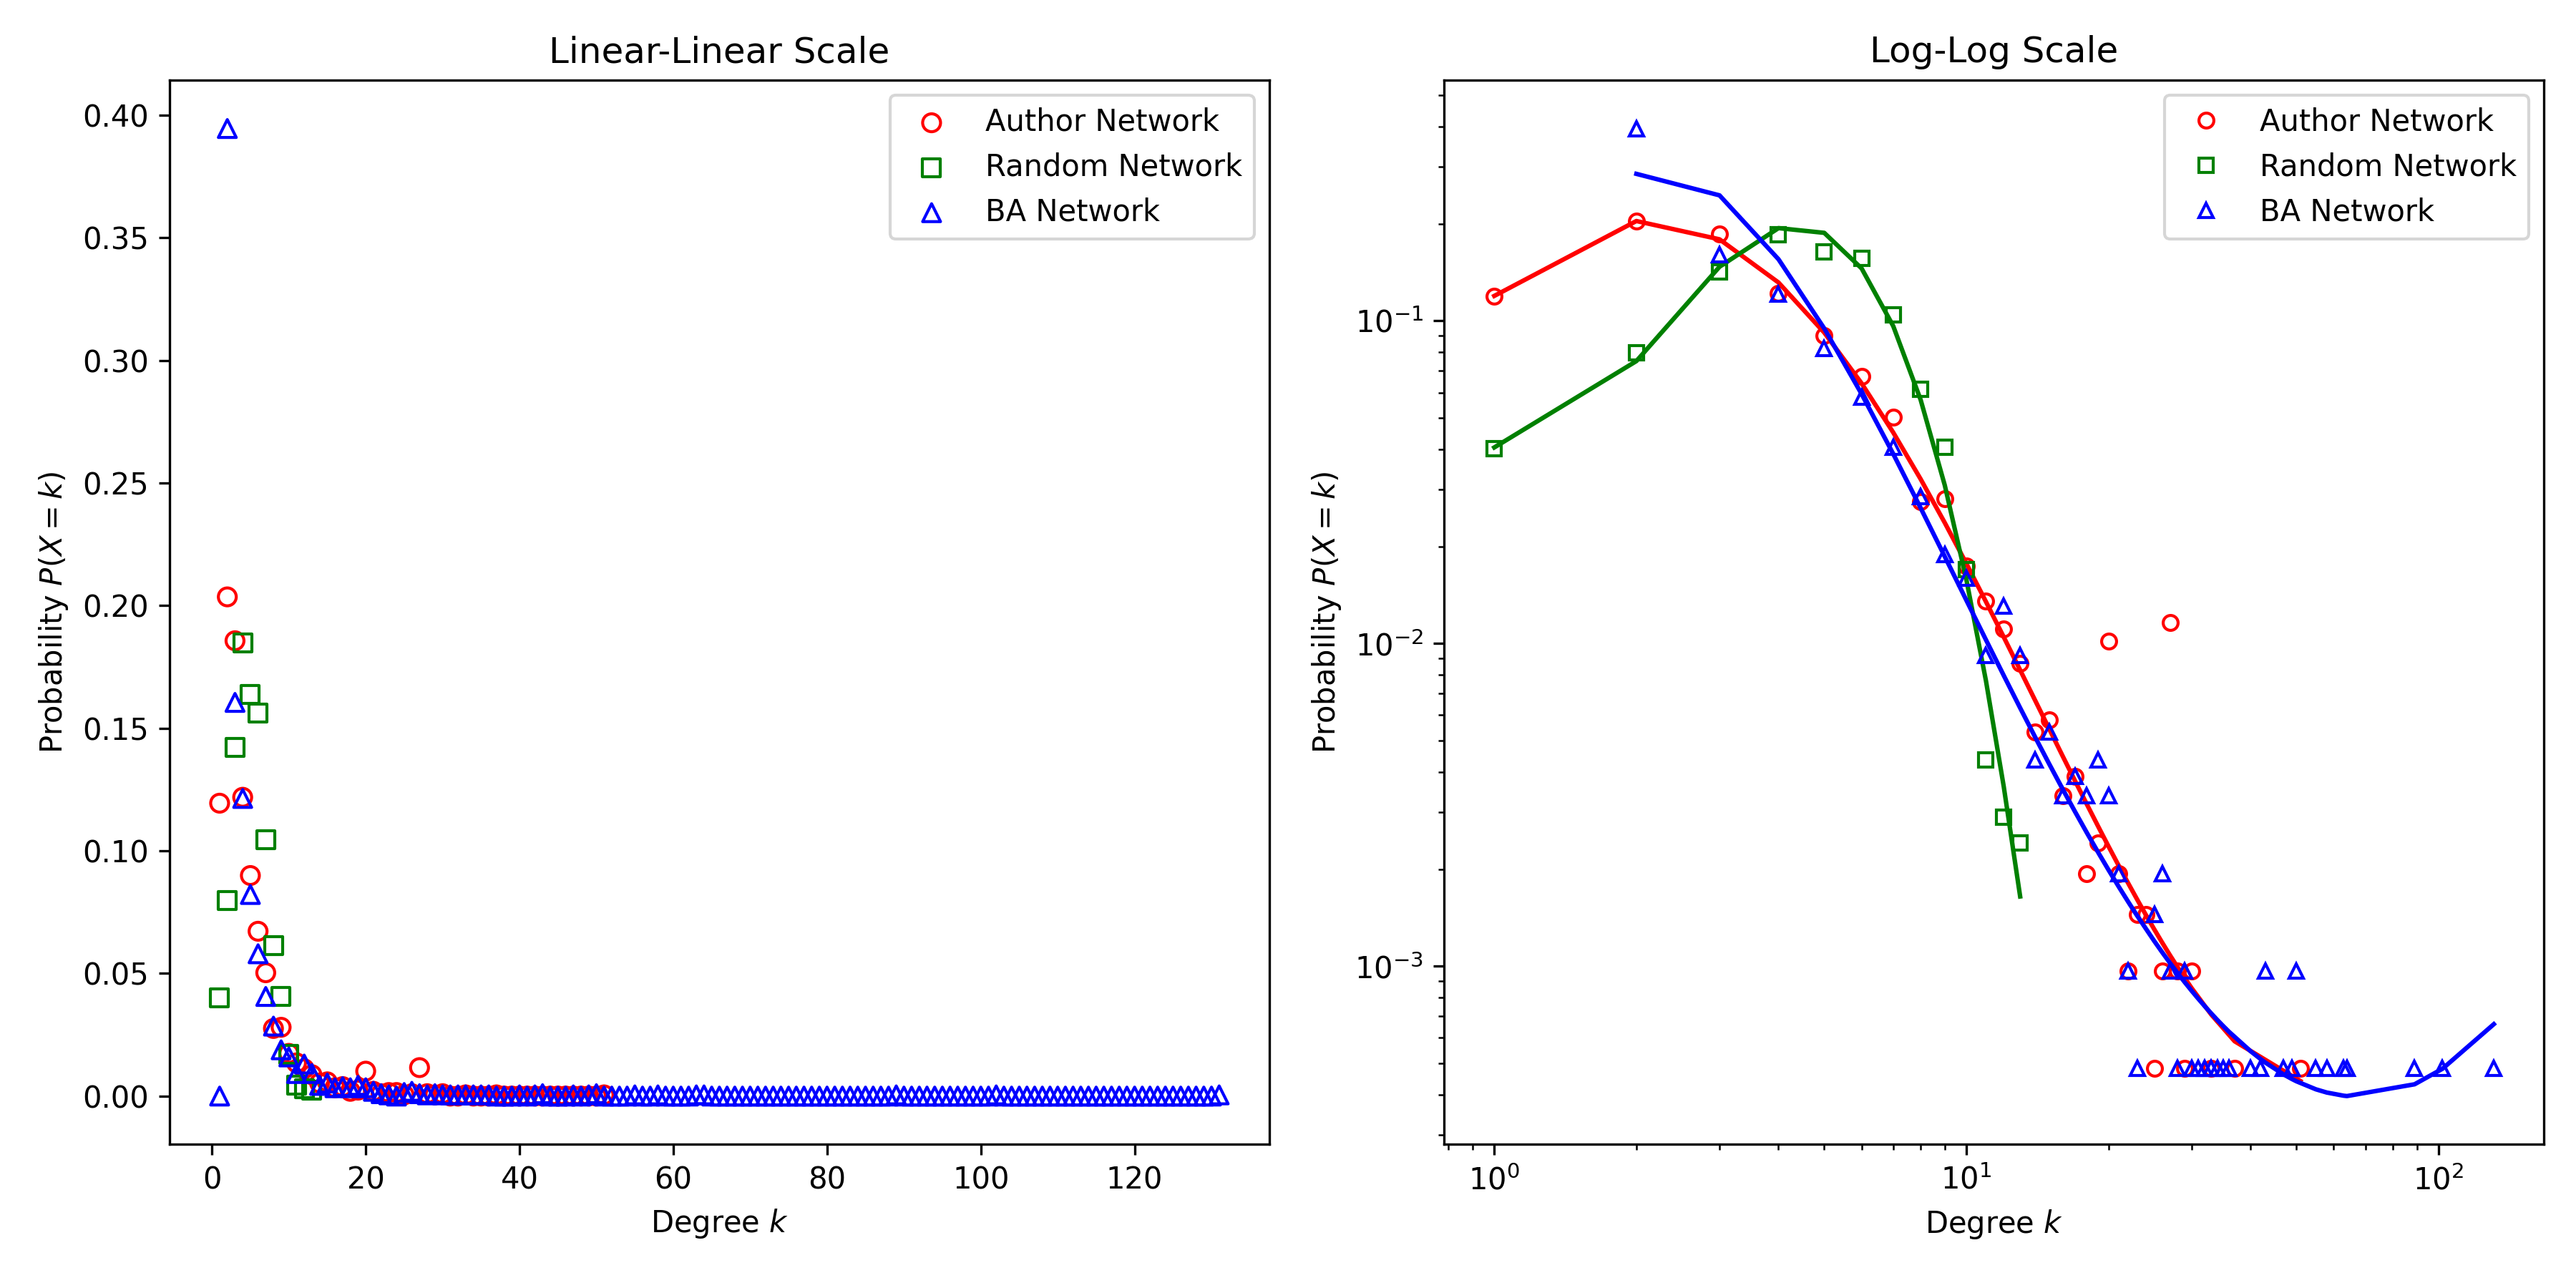
\includegraphics[width=1\textwidth]{degree_distributions.png}
    \label{fig:Degree_Distribution}
\end{figure}

\section*{Task 2 - (15 marks)}
\fbox{
  \parbox{1\textwidth}{
  \begin{itemize}
	\item Calculate and plot the nearest neighbour's average degree $k_{nn}$ as a function of degree $k$, on log-log scale.
	\item Calculate the assortative coefficient of the networks.
	\item Briefly discuss your results
\end{itemize}
  }
}

\begin{figure}[h]
    \centering
    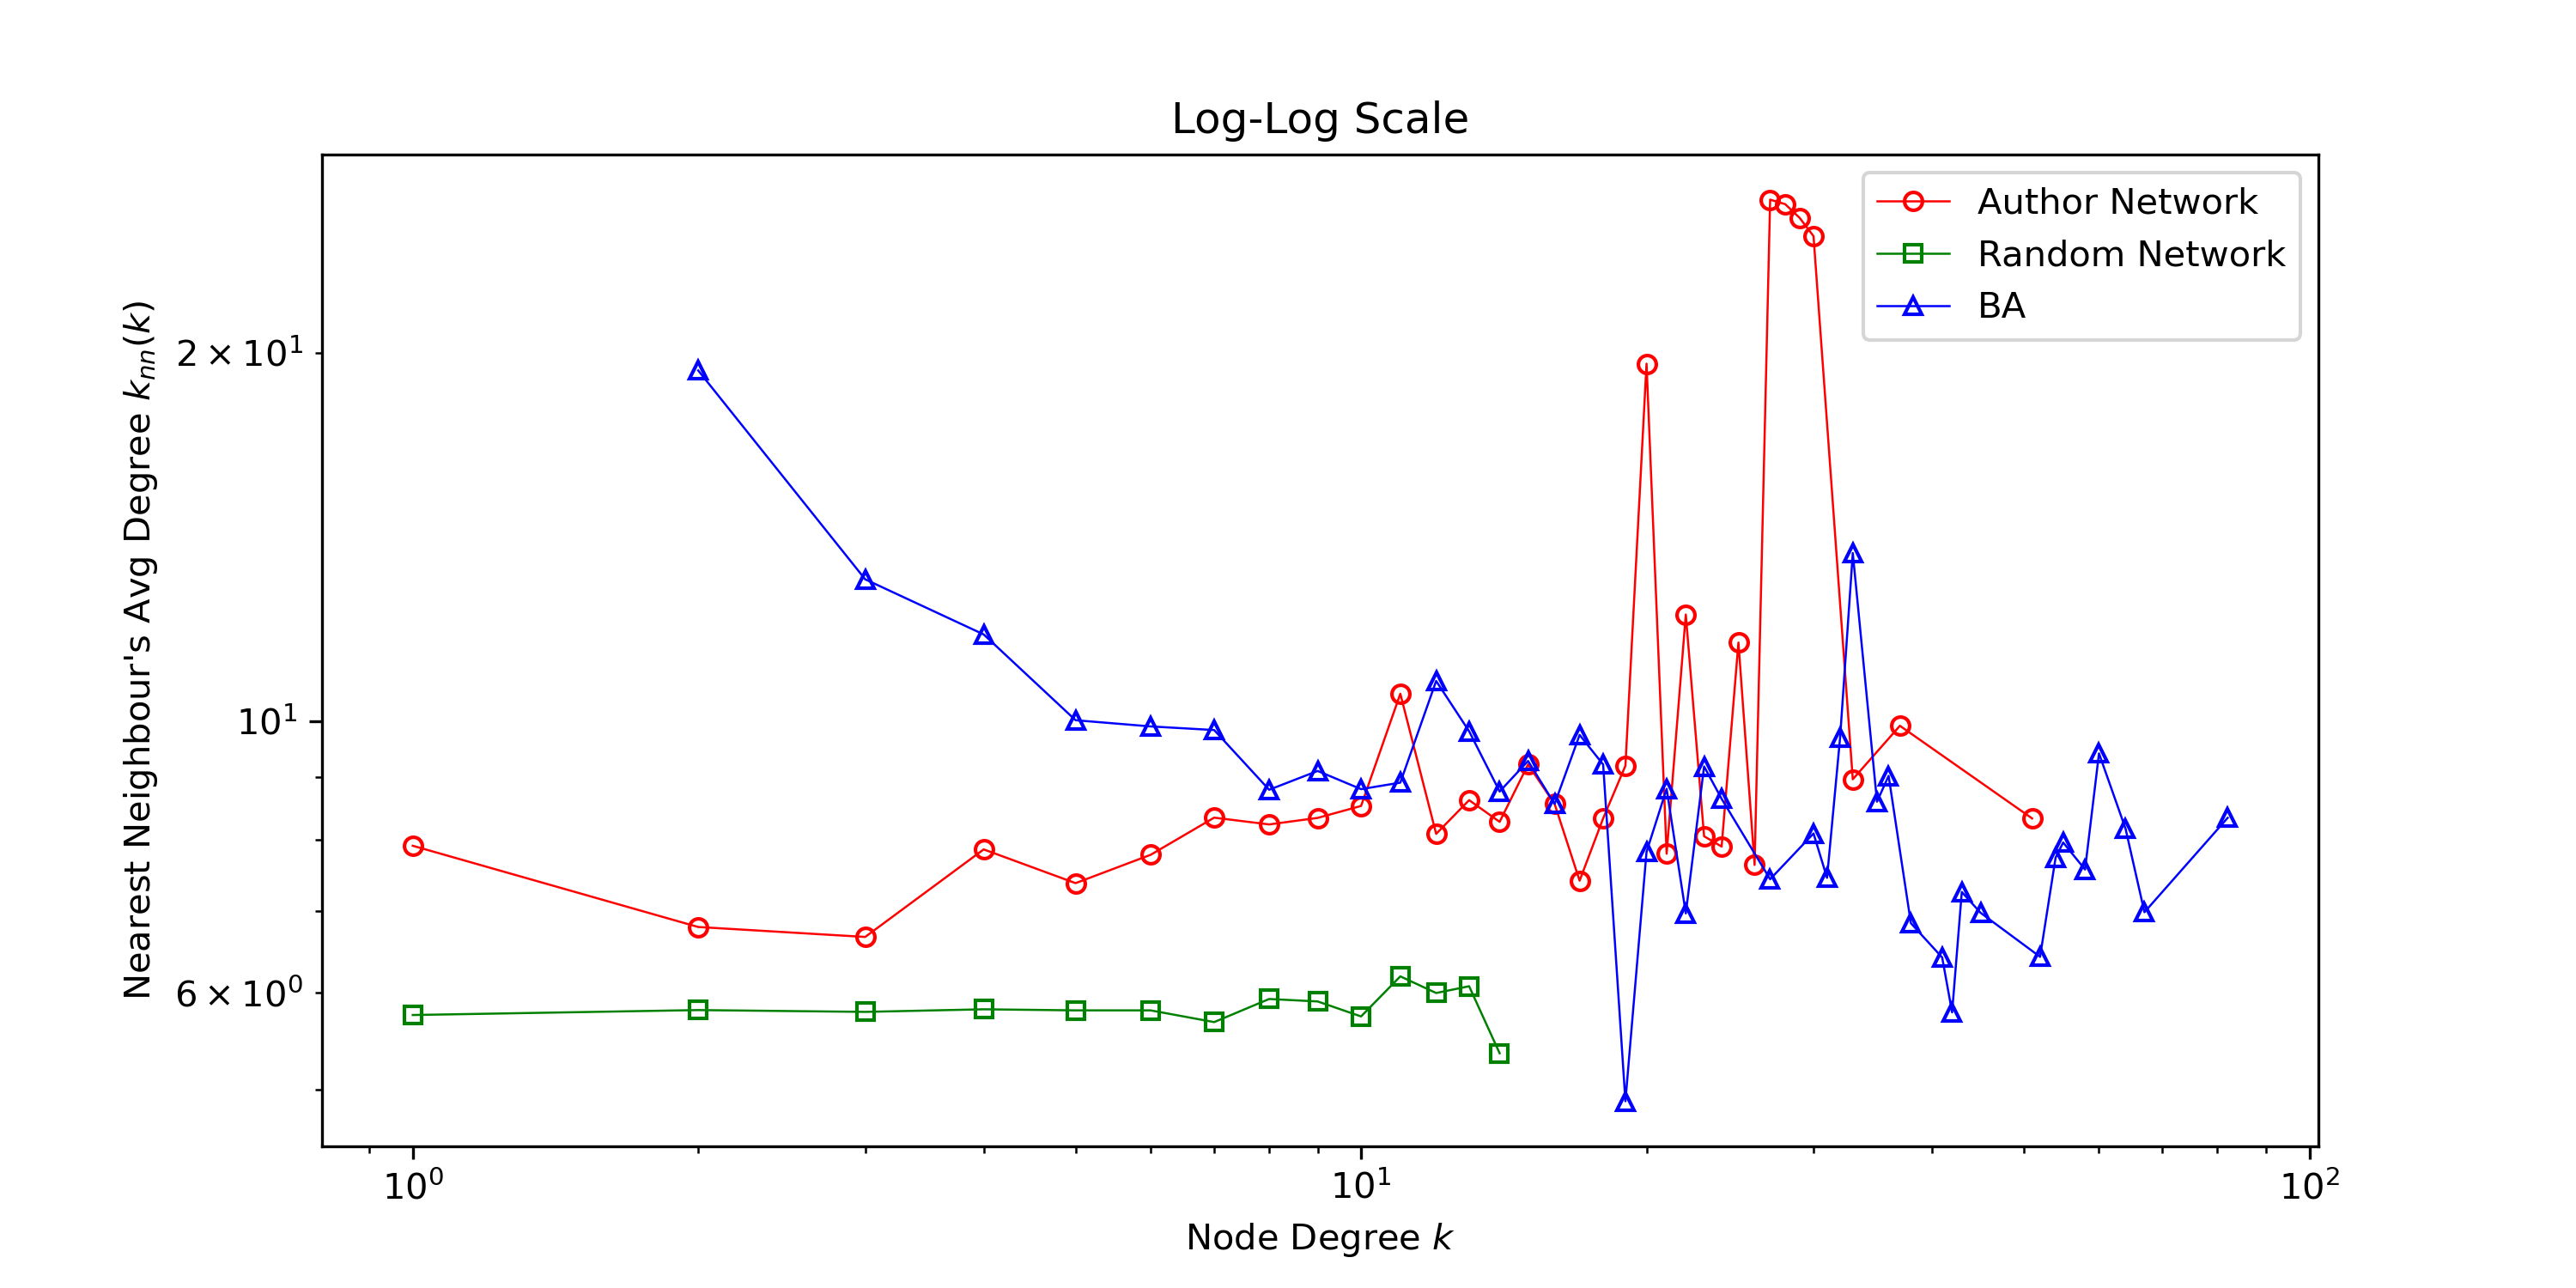
\includegraphics[width=1\textwidth]{nearest_neighbours_average_degree.png}
    \label{fig:Nearest Neighbours Average Degree}
\end{figure}

\begin{table}[h]
\centering
\begin{tabular}{lccc}
\toprule
& \textbf{Author Network} & \textbf{Random Network} & \textbf{BA Network} \\
\midrule
Assortative coefficient $\alpha$ & 0.47 & 0.01 & -0.09 \\
\bottomrule
\end{tabular}
\end{table}


\section*{Task 3 - (15 marks)}
\fbox{
  \parbox{1\textwidth}{
  	\begin{itemize}
	\item Calculate the diameter and the average shortest path length of the network
	\item Calculate and plot the average node between of $k$-degree nodes as a function of node degree $k$, where node betweenness is normalised, on log-log scale.
	\item Briefly discuss your results.
	\end{itemize}
  }
}

\begin{table}[h]
\centering
\begin{tabular}{lccc}
\toprule
 & \textbf{Author Network} & \textbf{Random Network} & \textbf{BA Network} \\
\midrule
Diameter $d$ & 19 & 10 & 7 \\
Average shortest path length $\ell$ & 7.30 & 4.97 & 4.18 \\
\bottomrule
\end{tabular}
\end{table}

\begin{figure}[h]
    \centering
    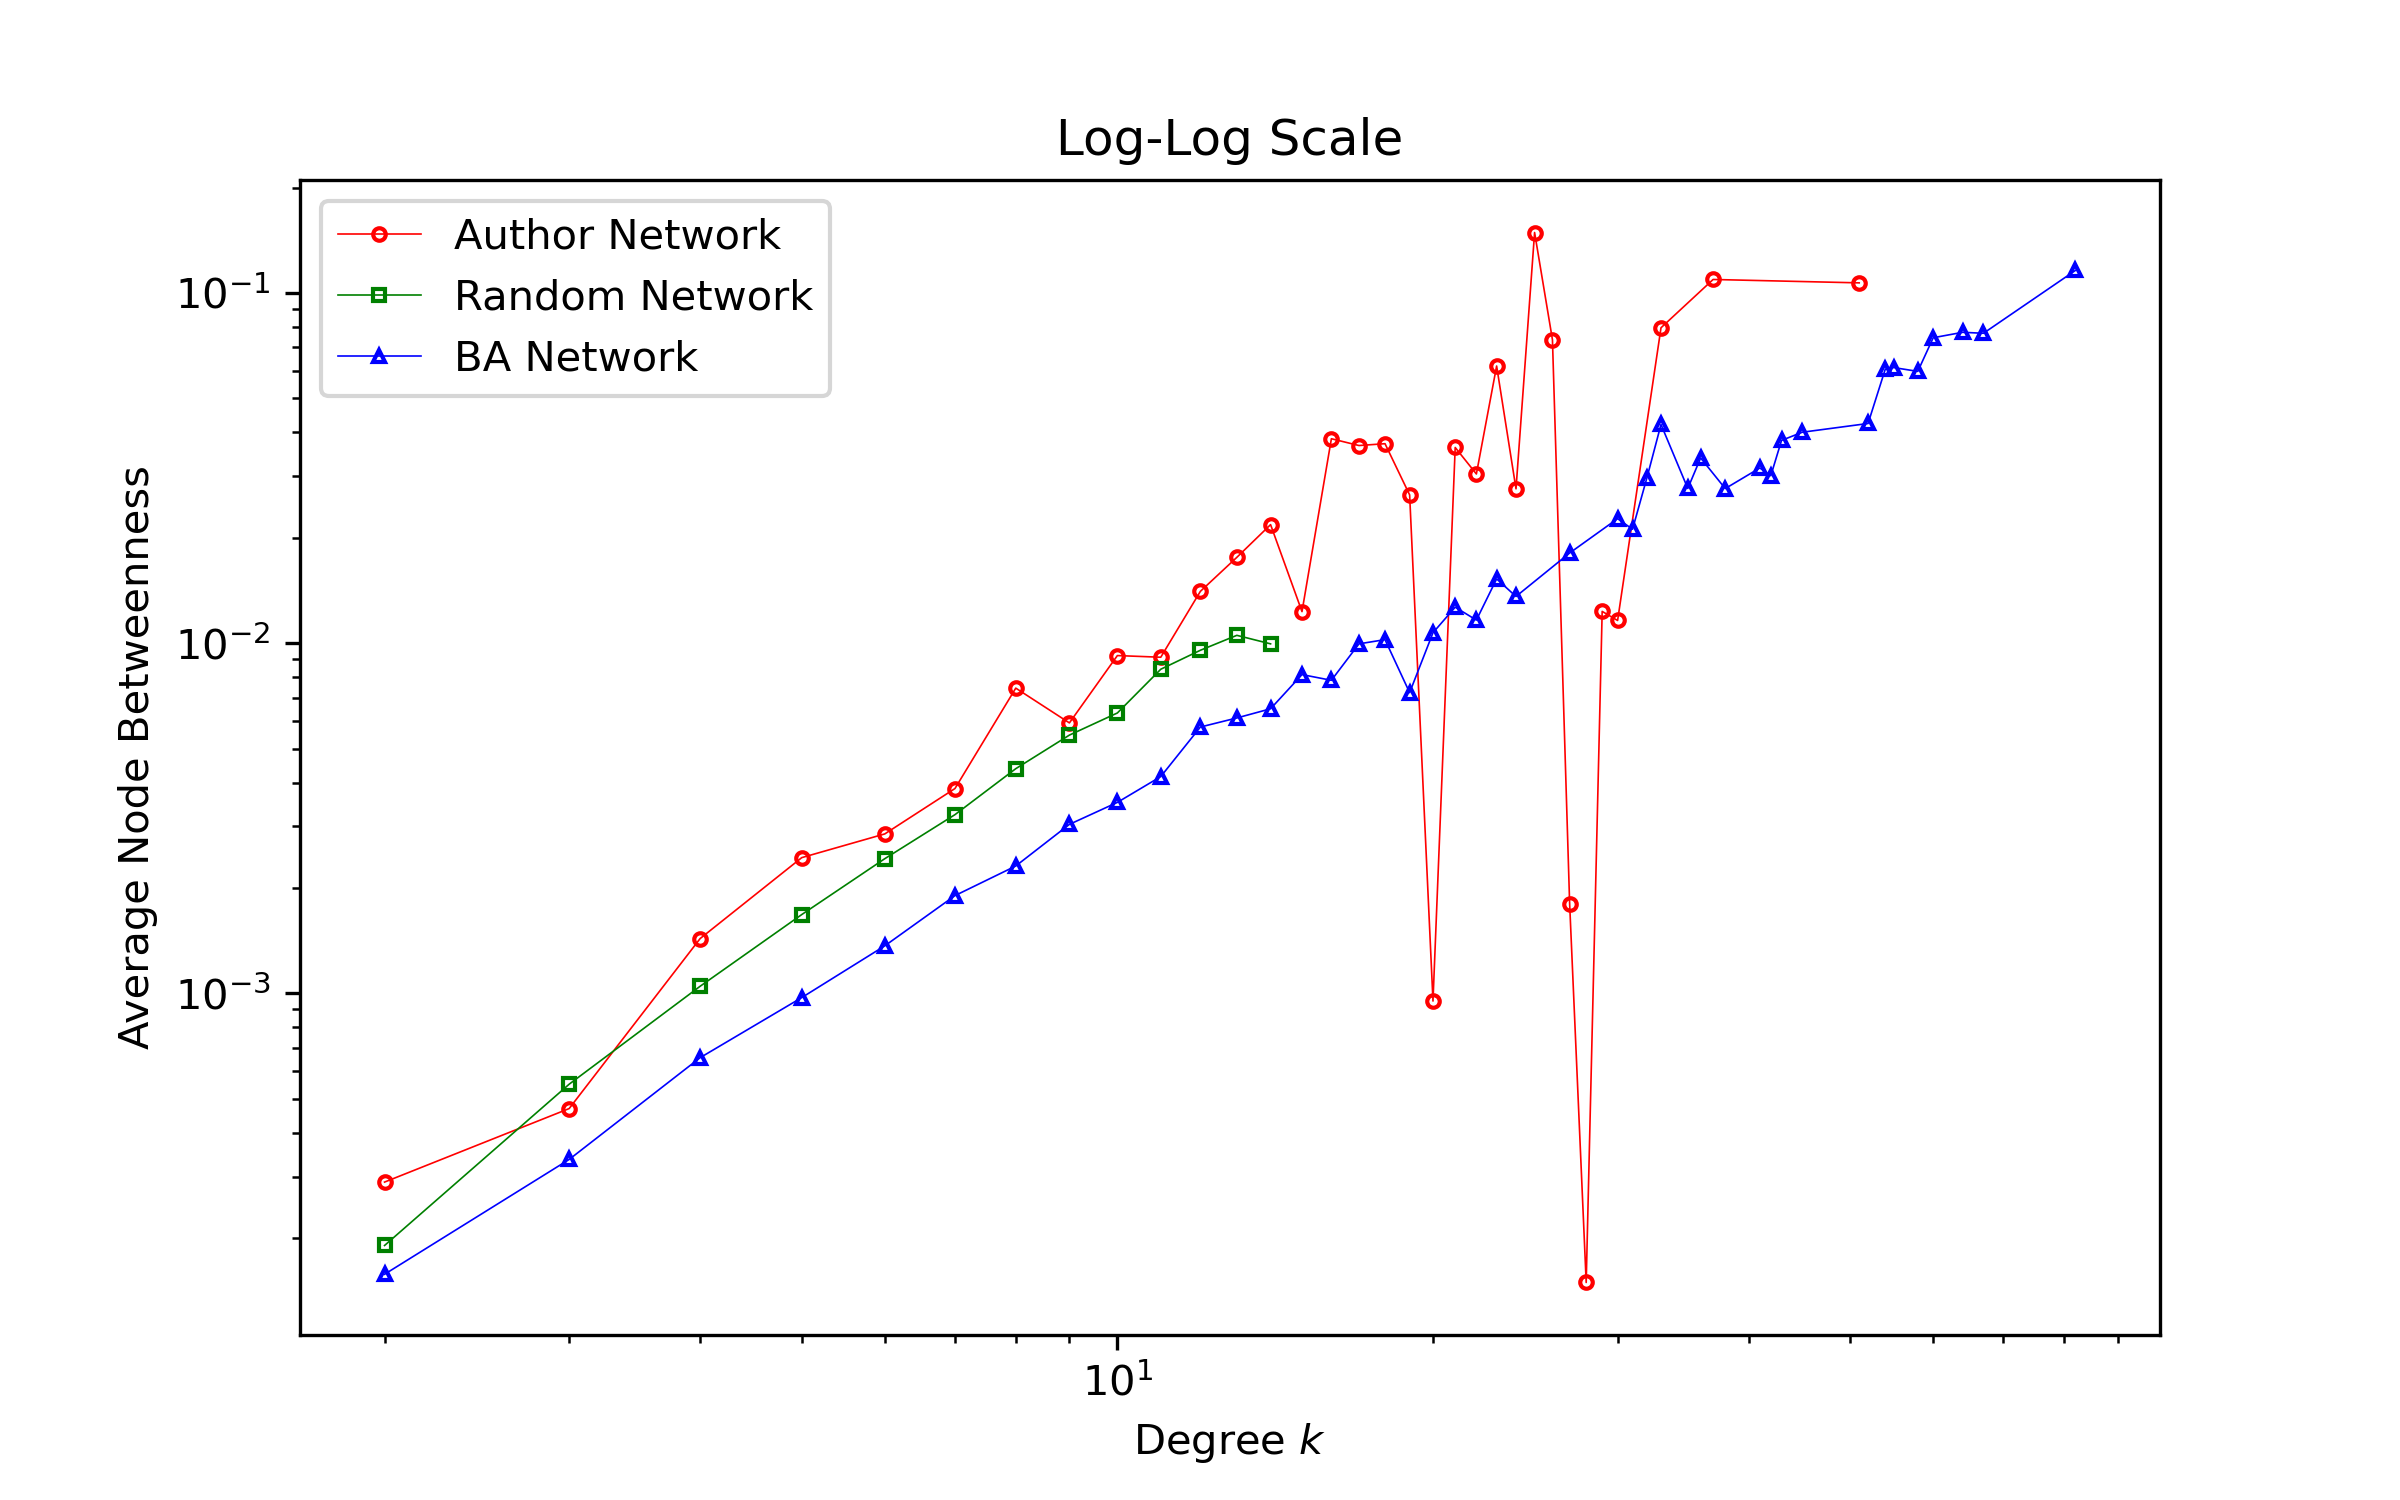
\includegraphics[width=1\textwidth]{average_node_betweenness.png}
    \label{fig:Averade Node Betweenness}
\end{figure}

\section*{Task 4 - (15 marks)}
\fbox{
  \parbox{1\textwidth}{
  \begin{itemize}
	\item Calculate and plot the rich-club coefficient as a function of node rank on log-log scale
	\item Calculate and plot the rich-club coefficient as a function of node degree on log-log scale
	\item Briefly discuss your result
\end{itemize}
  }
}

\begin{figure}[h]
    \centering
    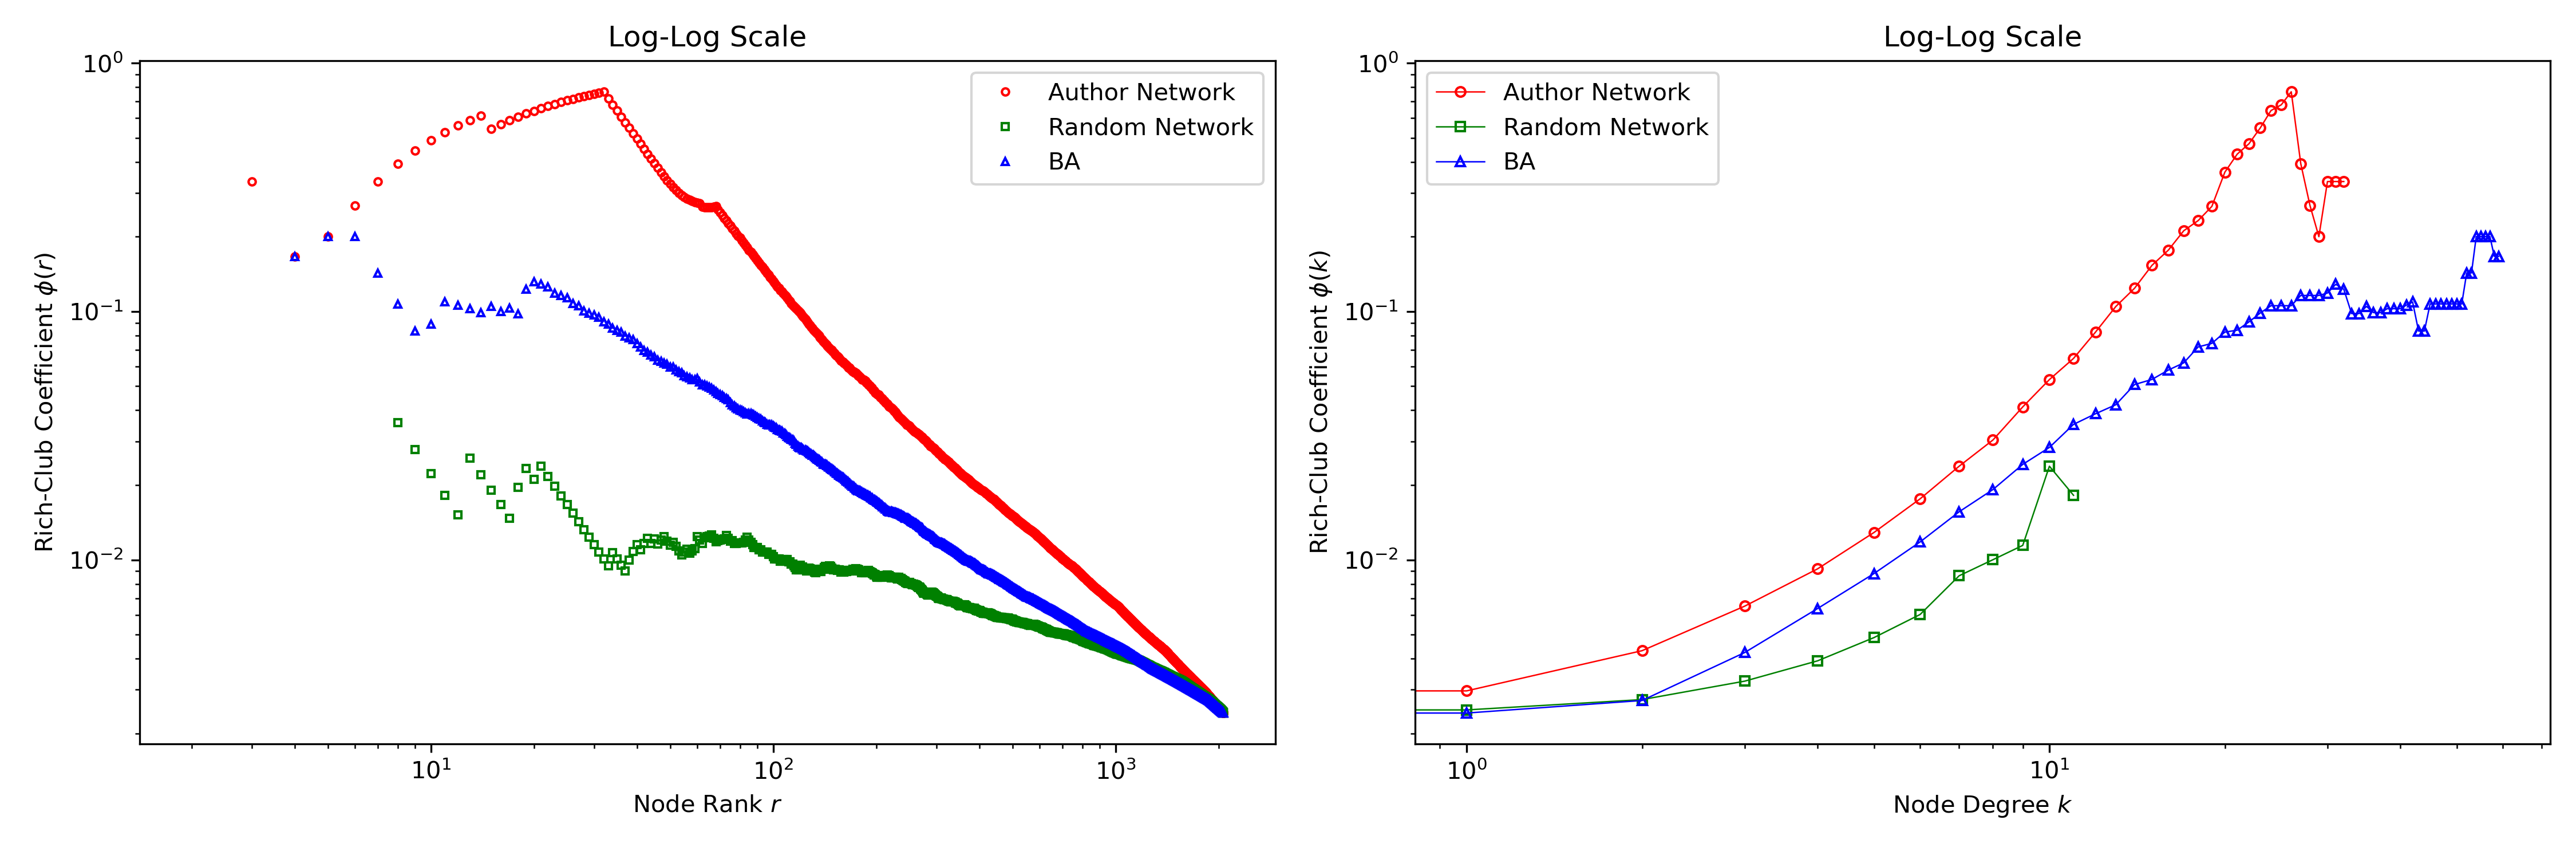
\includegraphics[width=1\textwidth]{rich_club.png}
    \label{fig:Rich-Club Coefficient}
\end{figure}

\section*{Task 5 - (15 marks)}
\fbox{
  \parbox{1\textwidth}{
  	\begin{itemize}
	\item Obtain the community structure (with the largest modularity value) of the 3 networks
	\item Give the number of communities and the size (i.e. number of nodes) of the top 3 largest communities in each netwoork.
	\item Visualise the 3 networks. In each network, show every community with a different colour.
	\item Briefly discuss your result
\end{itemize}
  }
}

\section*{Task 6 - (25 marks)}

\fbox{
	\parbox{1\textwidth}{
	\begin{itemize}
	\item Randomly rewire the 3 networks while preserving the degree distribution; and obtain the maximal random case of each network
	\item For the 3 randomised networks, plot their degree distribution
	\item For each of the randomised networks, calculate the average clustering coefficient, the assortative coefficient, the size of the giant component, and the average shortest path length in the giant component. Show these results and compare with those of the 3 original networks in a table,
	\item Briefly discuss your result.
\end{itemize}
	}
}

\begin{figure}[h]
    \centering
    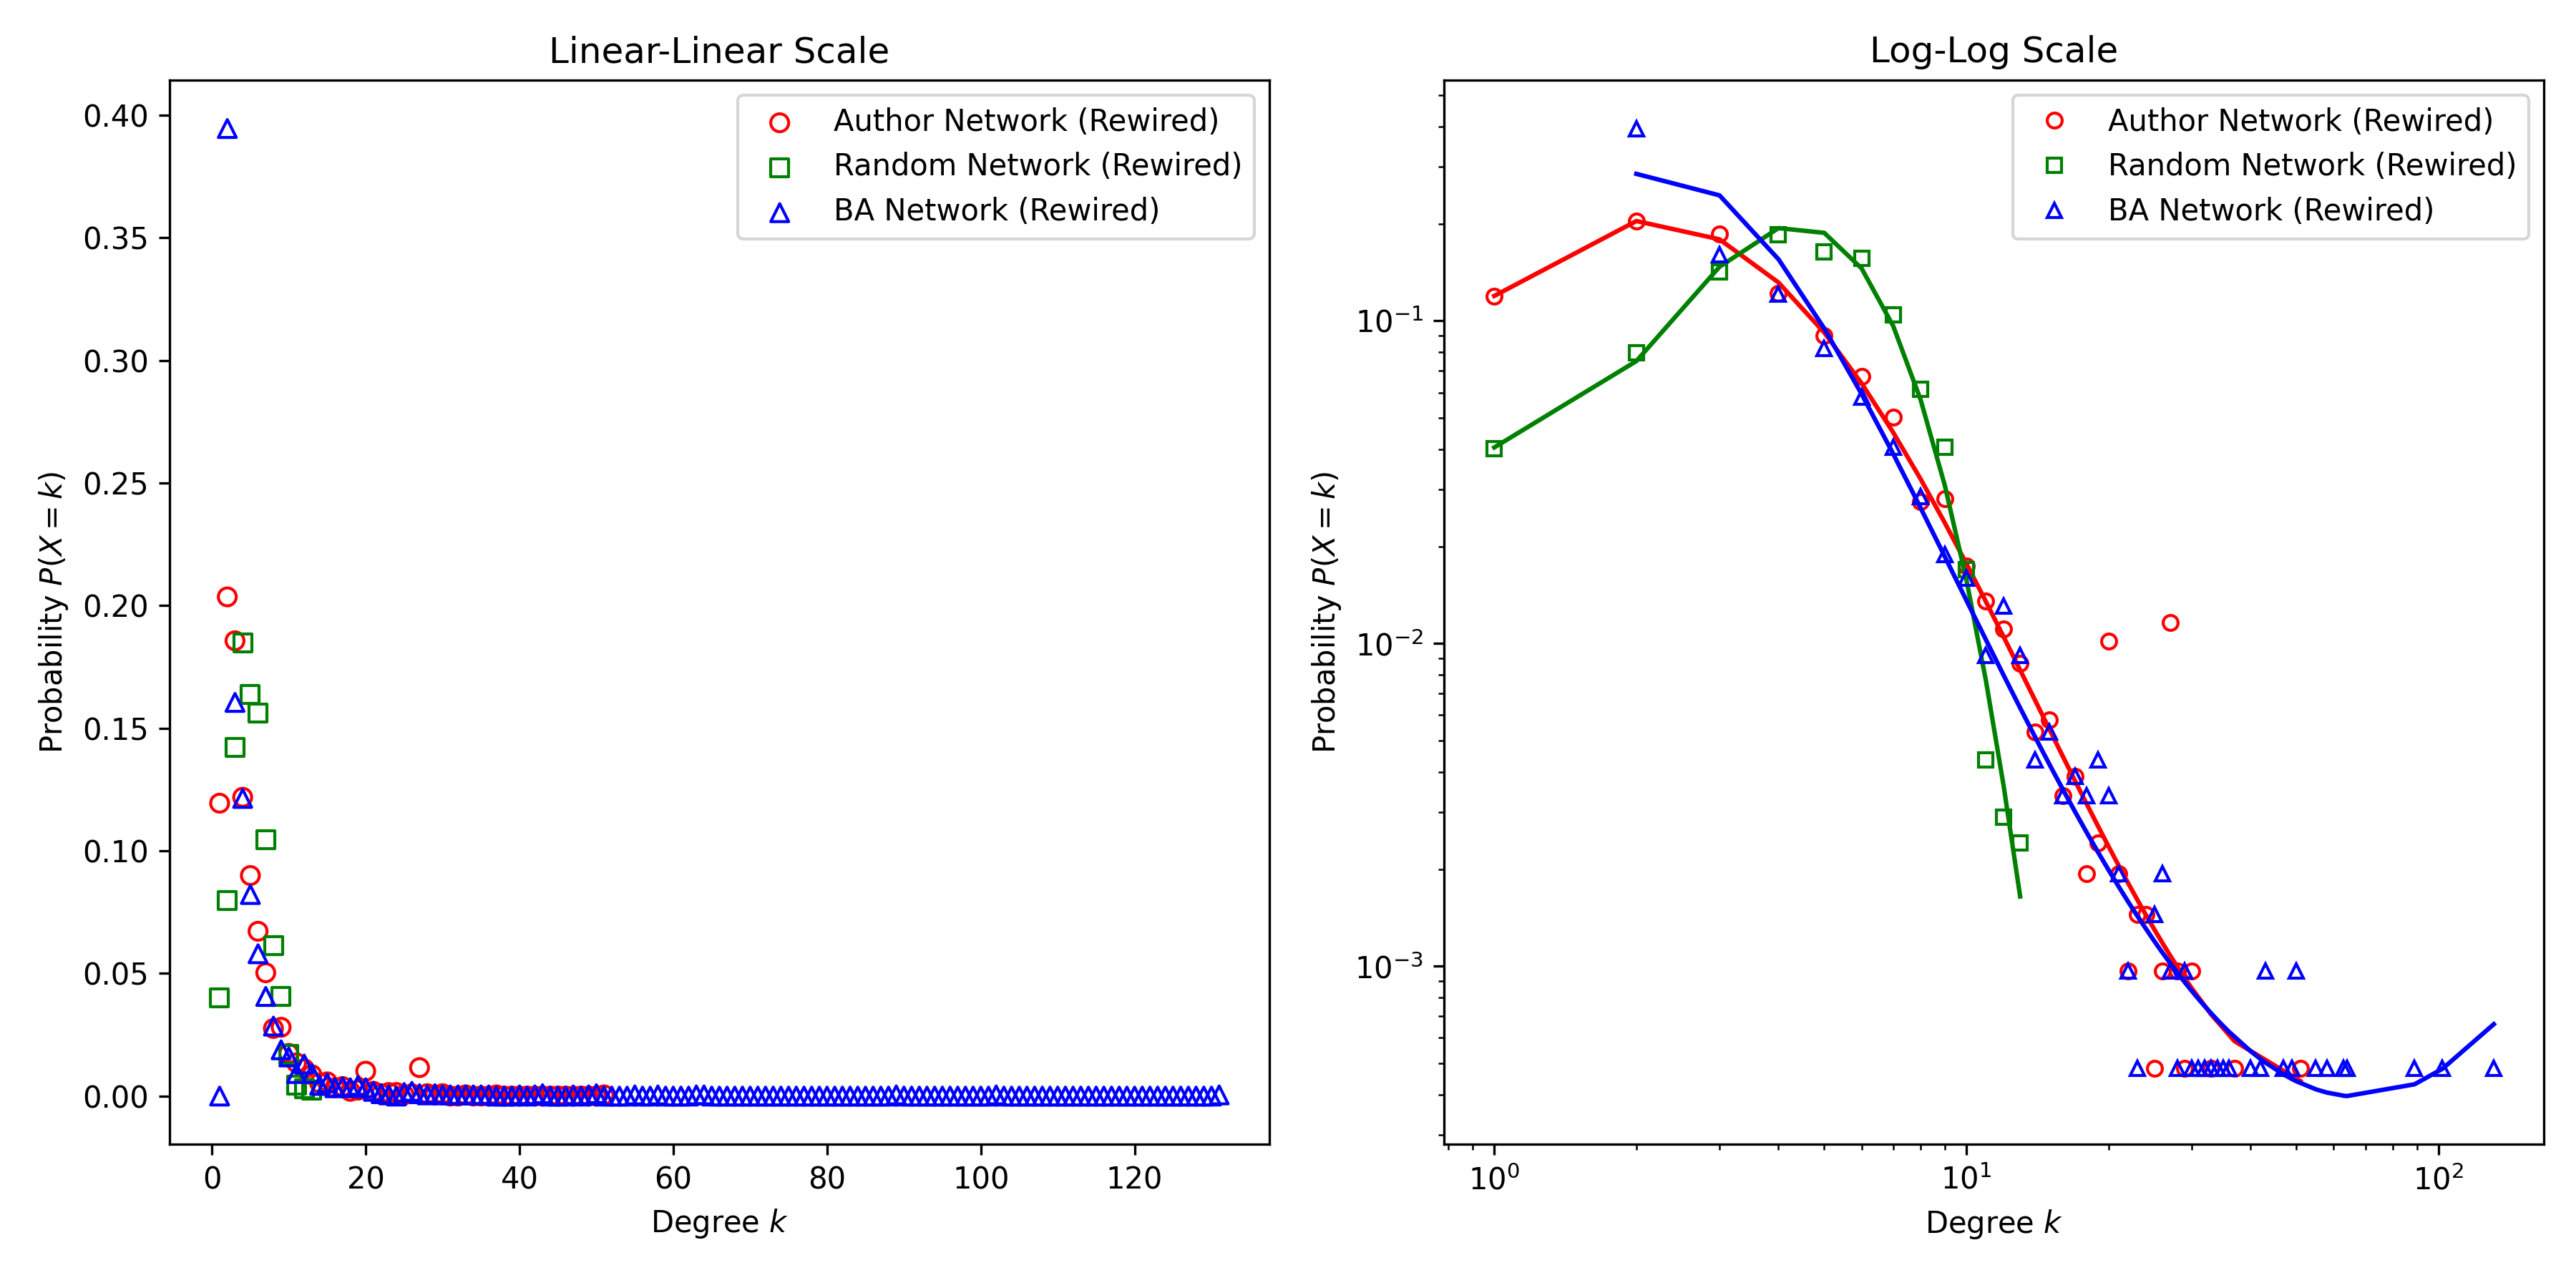
\includegraphics[width=1\textwidth]{degree_distributions_rewired}
    \label{fig:Degree Distributions (Rewired Networks)}
\end{figure}

\begin{table}[h]
\centering
\begin{tabular}{lccc}
\toprule
 \textbf{Original} & \textbf{Author Network} & \textbf{Random Network} & \textbf{BA Network} \\
\midrule
Giant Component Size $N$ & 2068 & 2068 & 2068 \\
Average Clustering Coefficient $C$ & 0.62 & 0.00 & 0.01 \\
Assortative coefficient $\alpha$ & 0.47 & 0.01 & -0.09 \\
Average shortest path length $\ell$ & 7.30 & 4.97 & 4.18 \\
\midrule
\textbf{Rewired} & & & \\
\midrule
Giant Component Size $N$ &  &  &  \\
Average Clustering Coefficient $C$ & 0.01 & 0.00 & 0.01 \\
Assortative coefficient $\alpha$ & 0.05 & 0.01 & -0.02 \\
Average shortest path length $\ell$ & 4.44 & 4.98 & 4.24 \\
\bottomrule
\end{tabular}
\end{table}

\newpage
\bibliographystyle{acm}
\bibliography{references}

\end{document}